\documentclass{article}

\usepackage{mathrsfs,amsmath}
\usepackage{xcolor}
\usepackage{titlesec}
\usepackage{listings}
\usepackage{syntax}
\usepackage{pythonhighlighting}
\usepackage{graphicx}

\graphicspath{ {./assets/} }

\usepackage[margin=1.4in]{geometry}

\title{Project \#1 Write Up | CS 335} 
\author{Jared Dyreson\\ 
        California State University, Fullerton}

\DeclareRobustCommand{\bowtie}{%
  \mathrel\triangleright\joinrel\mathrel\triangleleft}


\usepackage [english]{babel}
\usepackage [autostyle, english = american]{csquotes}
\MakeOuterQuote{"}

\titlespacing*{\section}
{0pt}{5.5ex plus 1ex minus .2ex}{4.3ex plus .2ex}
\titlespacing*{\subsection}
{0pt}{5.5ex plus 1ex minus .2ex}{4.3ex plus .2ex}

\usepackage{hyperref}
\hypersetup{
    colorlinks,
    citecolor=black,
    filecolor=black,
    linkcolor=black,
    urlcolor=black
}

\begin{document}

\maketitle
\tableofcontents

\newpage

\section{General Information}

\subsection{Contributors}

\begin{enumerate}
\item Jared Dyreson | \href{mailto:jareddyreson@csu.fullerton.edu}{\underline{jareddyreson@csu.fullerton.edu}}
\end{enumerate}

\subsection{Repository}

The repository for this project can be found \href{https://github.com/JaredDyreson/Matching-Schedules}{\underline{here}}

\subsection{Linux Screenshot}

\begin{figure}[!h]
\centering
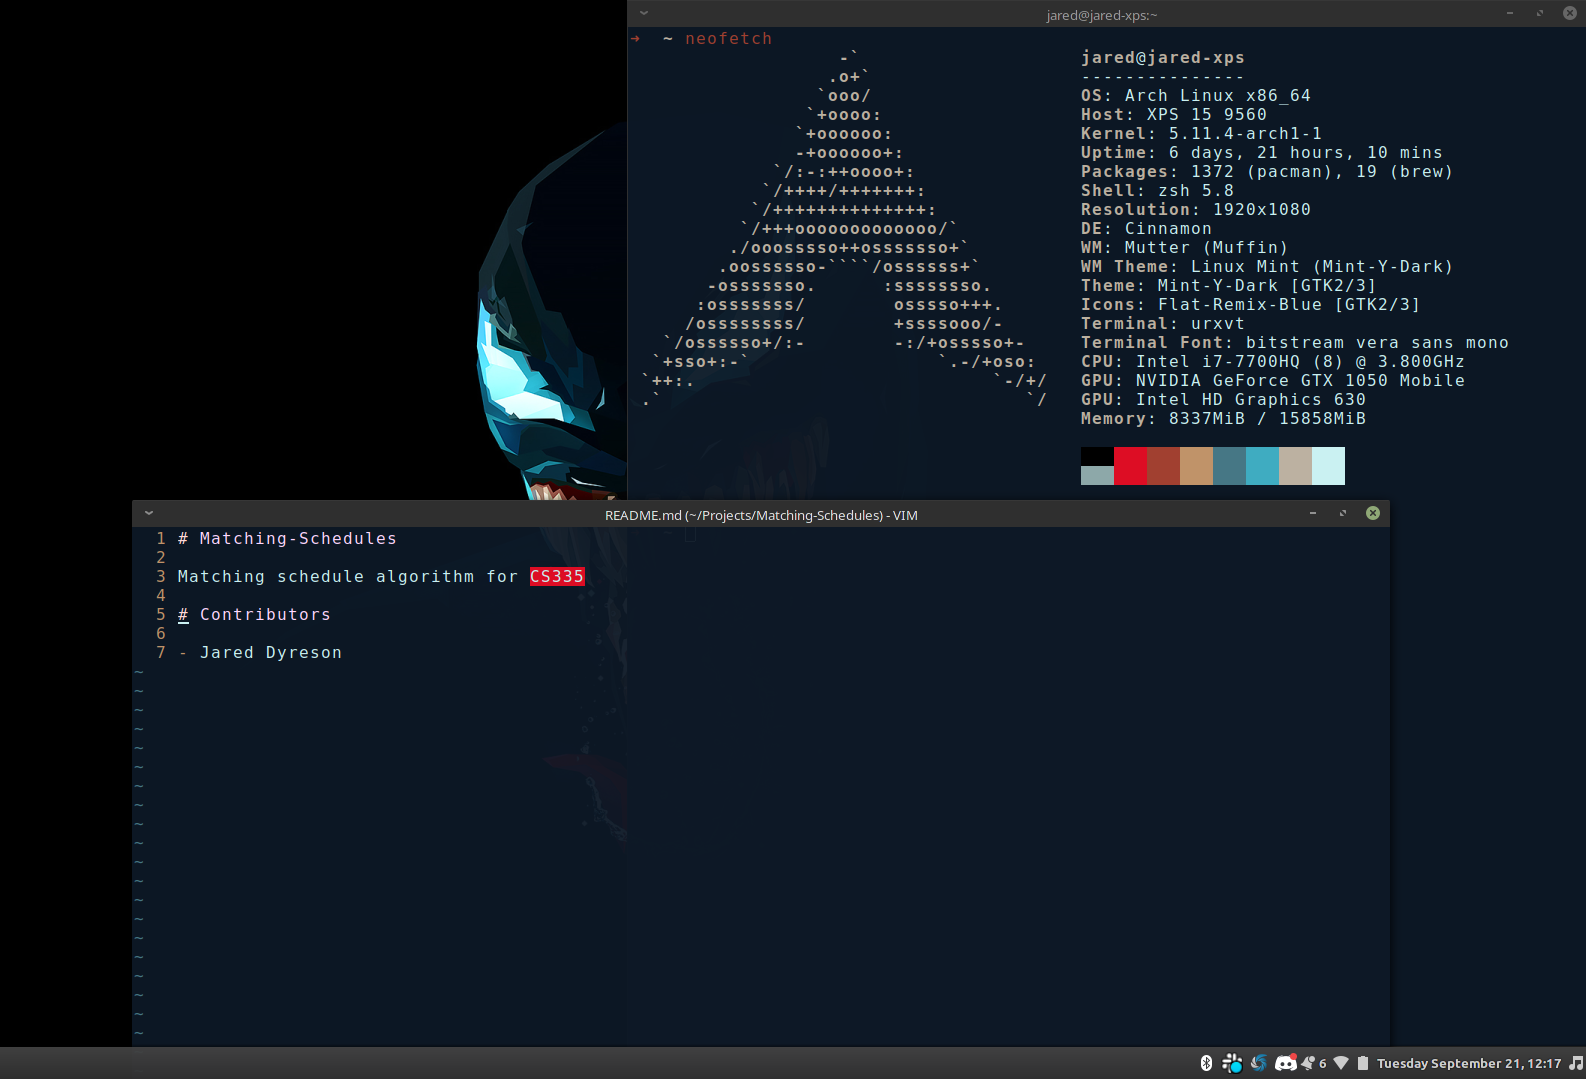
\includegraphics[width=16cm]{arch_linux}
\end{figure}

\newpage

\section{Pseudocode}

\textbf{NOTE:} time complexity of reading input files is not calculated in this write up. This algorithm assumes that the data is in the proper format when ingested and is available in constant time.


\subsection{combineSchedule}

\begin{verbatim}
function combineSchedule(person1, person2):
   container = [] // empty list (1)
   longer_schedule = max(len(schedule_a), len(schedule_b)) // 1
   for each element in both schedules: // 2 atomics (2n)
       // this if statement is considered "n + 1"
       if element is not present in the container: // "n" atomics
           insert into container // 1 atomic

    // above for loop is: (2n + 2) * (n + 1) => 2n^2 + 4n + 2

   for remaining elements in longer_schedule: 
       // 2 atomics (assuming assignment and incrementing index counter)

       if element is not present in the container: // "n" atomics
            insert into the container // 1
   
   // above for loop is: (2n) * (n + 1) => 2n^2 + 2n

   sort container based on the beginning element in the interval
   // assuming sorting algorithm is implemented in n * log(n) time
   return container // 1

\end{verbatim}


\subsubsection{Analysis}

This function primarily is going to combine two lists into one larger list.
It is not required that both lists have the same length and in the overall analysis of this function, it does not matter.
If we add up each individual instruction, we get:
$$ 2n^{2} + 4n + 3 + 2n^{2} + 2n + n \times \log(n)$$
$$ 4n^{2} + 6n + n \times \log(n) + 3$$
Our overall time complexity will be in $O(4n^{2}) \implies O(n^{2})$, as it is the leading term in this polynomial equation.
In this instance, we can do better if we utilize an ordered set because we do not have to constantly check the container if the element is present.
We can also use a dictionary/hash set to accomplish the same goal, as duplicates are ignored.
Lastly, we could have ignored the duplicates and have themselves be combined into one large interval later in the program.
With the current algorithm, it is unknown if this will work as intended.


\newpage

\subsection{mergeSchedules}

\begin{verbatim}
function mergeSchedules(person1, person2):
    result = combineSchedule(person1, person2) # 1 (assume data is ready in constant time)
    if no result: # 1
        return empty list # 2 (instantiate list, then return)
    
    stack = new Stack # 1

    stack.push(result[0]) # 1
    # (2 atomics, assignment and increment index)
    for slot in result[1:]: # everything after 0th index 
        top = stack.peek() # 1
        
        if(top.end < slot.begin): # place a new interval onto the stack (1)
            stack.push(slot) # 1
        else: (1)
            top.end = max(top.end, slot.end) # up date the end of the current interval (1)
    # loop : 4 atomics
    
    return stack in reverse order # n + 1; you need to unwind the stack

\end{verbatim}

\subsubsection{Analysis}

In mergeScheudles, it will attempt to combine several separate time intervals into smaller, contiguous intervals.
For example, the two intervals "00:00$\rightarrow$09:00" and "09:00$\rightarrow$10:30" will be returned as "00:00$\rightarrow$10:30".
However, if we include the new interval "12:00$\rightarrow$14:00", we will now have two separate yet contiguous intervals: "00:00$\rightarrow$10:30", "12:00$\rightarrow$14:00".
When we add up each individual instruction, we get the following: \\
$$6 + 6n + n + 1$$
$$7n + 7$$
This will eventually decay to $O(n)$, which is the best case we can get given our constraints for this problem.
We could improve the space complexity by implementing the stack using a standard list in Python.
This would alleviate having to unwind the stack and putting that data into another container.

\newpage

\subsection{dispenseTime}

\begin{verbatim}
function dispenseTime(mergedInterval):
    edge_one, edge_two = mergedInterval[0][1], mergedInterval[-1][0] # 2
    container = [] # 2
    # 2 atomics (assignment and increment)
    for element in mergedInterval ignoring first and last index:
        begin, end = element.begin, element.end # 2, unpacking values of element
        container.append(begin) # 1
        container.append(end) # 1
    # loop : 6n

    container insert at first index the first edge case # 1
    container append last edge case # 1
    return list that is evenly paired together # n
    // [[1, 2], [2, 4]]

\end{verbatim}

\subsubsection{Analysis}

In this function, we are interested in pairing up the intervals given from mergeSchedules.
The aforementioned function does not remove edge cases wherein either client cannot attend a meeting.
Since all intervals are not contained in a contiguous block, we are forced to iterate over all of them and remove two time slots.
One way to alleviate this would be to have some sort static inline container holding pointers to all the time interval class instances.
For example:

\begin{verbatim}
  // code dervied from CS 462 : Thomas Bettens
  protected:
    // Enable derived classes to register themselves into a collection of people
    Person()
    { people.insert( this ); }

    inline static std::set<Person *> people;  // collection with no duplicates
\end{verbatim}

\begin{flushleft}
Given this project was implemented in Python, we have no concept of pointers.
To compute the time complexity, we will add up the individual instructions:

$$4 + 6n + n + 2$$ \\
$$7n + 6$$

Which eventually decays to $O(n)$.

\end{flushleft}

\end{document}

